\documentclass[convert={size=280x210}]{standalone}
\usepackage[utf8]{inputenc}
\usepackage{tikz}
\usetikzlibrary{calc, decorations.markings}
\usepackage{siunitx}
\sisetup{locale=FR, per-mode=symbol}

\begin{document}
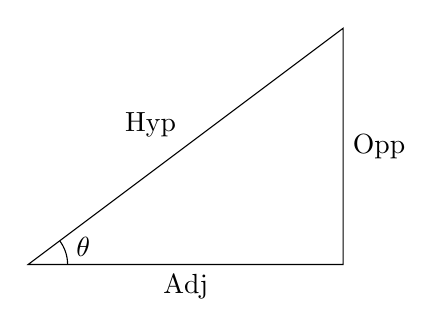
\begin{tikzpicture}[>=stealth, scale=1]
  \coordinate (A) at (0, 0);
  \coordinate (B) at (4, 0);
  \coordinate (C) at (4, 3);
  \draw (A) -- node[below] {Adj}
        (B) -- node[right] {Opp}
        (C) -- node[anchor=south east] {Hyp} cycle;
  \draw ($(A) + (0.5, 0)$) arc (0:36.87:0.5);
  \node at ($(A) + (0.7, 0.22)$) {$\theta$};
\end{tikzpicture}
\end{document}
